\documentclass{jsarticle}
\usepackage[dvipdfmx]{graphicx}
\usepackage{amsmath,amssymb}
\usepackage{amsmath}
\usepackage{mathtools}
\mathtoolsset{showonlyrefs=true}

\title{やさしく学ぶ機械学習を理解するための数学のきほん}

\begin{document}
\maketitle

\section{分類}
画像の縦横のサイズだけをみて、縦長なのか横長なのかを判断する二値分類を考える。

例えば以下のようなデータが有ったとする。

\begin{table}[htb]
  \begin{tabular}{|l|c|r|} \hline
    縦 & 横 & 形 \\ \hline
    50 & 10 & 縦長 \\ \hline
	20 & 40 & 横長 \\ \hline
	10 & 20 & 横長 \\ \hline
	40 & 30 & 縦長 \\ \hline
	25 & 45 & 横長 \\  \hline
	45 & 25 & 縦長 \\ \hline
  \end{tabular}
\end{table}

\begin{center}
  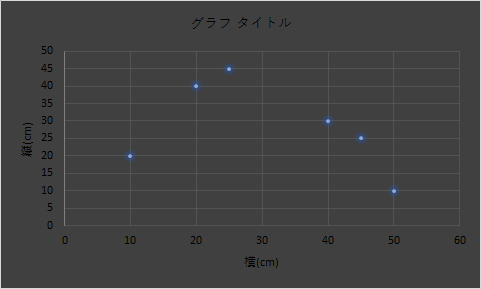
\includegraphics[width=15cm]{figures/graph.png}
\end{center}

このとき「縦長」と「横長」を二分する線を引くとすると以下のような線が引ける

\begin{center}
  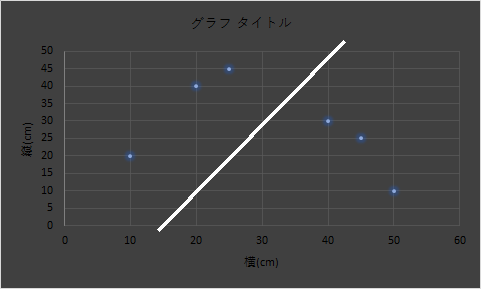
\includegraphics[width=15cm]{figures/graph2.png}
\end{center}

分類の目的はこのような線を見つけることにある。

\subsection{内積}
線を見つけることが目的だが、回帰でやった1次関数の傾きと切片を求めるのではなく、ベクトルを見つけることを目的とする。

先程データを分類するために引いた線は、\bf{重みベクトル}を\bf{法線ベクトル}とする直線になる。重みベクトルを$\bf{w}$とすると、その直線の方程式は以下のように表すことができる。

\[
	\bf{w} \cdot \bf{x} = 0
\]

重みベクトルは要するに、知りたいパラメータのことで、\bf{w}は「重み」を英語で表した頭文字。

内積は、実ベクトルの各要素の積を足し上げたものだから、上記の式は以下のように書くことができる。

\[
	\bf{w} \cdot \bf{x} = \sum_{i=1}^{n} w_{i} x_{i} = 0
\]

いまは縦と横の2次元で考えるから

\[
	\bf{w} \cdot \bf{x} = w_1 x_1 + w_2 x_2 = 0
\]

とかける。

法線は、ある直線に対して垂直なベクトルのこと。例えば重みベクトルを$w = (1,1)$としたら

\begin{align}
	w \cdot x &= w_1 x_1 + w_2 x_2 \\
    &= 1 \cdot x_1 + 1 \cdot x_2 \\
    &= x_1 + x_2 = 0
\end{align}

これにより$x_2 = -x_1$と書くことができ、これは重みベクトル$w=(1,1)$と垂直の線となる。これが「重みベクトルを法線ベクトルとする直線」に相当する。

また、内積のベクトル同士の成す角$\theta$とcosを使った

\begin{align}
	w \cdot x = |w| \cdot |x| \cdot \cos \theta
\end{align}

という四季でも表すことができる。$|w|と|x|$は必ず正になるので、内積が0ということは$\cos \theta = 0$ということ。$\cos \theta = 0$になるということは$\theta = 0^\circ か \theta = 270^\circ$になるということ。

最終的に、グラフに引いた直線に対して直角になる重みベクトルを見つけていけば良いことになる。重みベクトルを学習によって見つけると、そのベクトルに対して血垂直な直線がわかって、その直線によってデータが分類できる、という流れ。

\subsection{パーセプトロン}
では、具体的に動のようにして重みベクトルを求めていくのか。

基本的には回帰でやったように、重みベクトルをパラメータとして、更新式を作ってパラメータを更新していく。これから説明するものは「パーセプトロン」と呼ばれるもの。

パーセプトロンは複数の入力を受け取ってそれぞれの値に重みをかけて耐上げたものが出力されるというモデルっで、以下のような図でよく表される。

\begin{center}
  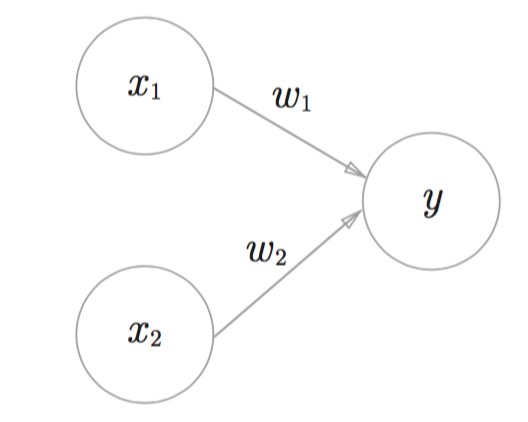
\includegraphics[width=15cm]{figures/graph3.png}
\end{center}

パーセプトロン自体は非常に単純なモデルなので実用されることはないが、ニューラルネットワークやディープラーニングの考え方のもとになっている。

パラメータ更新式の前rに、いくつかの前準備が必要となるので次で見ていく。

\subsubsection{学習データの前準備}
学習データについて、横幅を$x_1$、縦幅を$x_2$、横長・縦長については、横長を-1、縦長を1としてyで表すことにする。表にすると次のようになる。

\begin{table}[htb]
  \begin{tabular}{|r|r|r|r|r|} \hline
    画像サイズ & 形 & x1 & x2 & y \\ \hline
    80×150 & 縦長 & 80 & 150 & -1 \\ \hline
    60×110 & 縦長 & 60 & 110 & -1 \\ \hline
    35×130 & 縦長 & 35 & 130 & -1 \\ \hline
    160×50 & 横長 & 160 & 50 & 1 \\ \hline
    160×20 & 横長 & 160 & 20 & 1 \\ \hline
    125×30 & 横長 & 125 & 30 & 1 \\ \hline
  \end{tabular}
\end{table}

そしてベクトルxを与えると、横長か縦長を判定する関数、つまり1か-1を返す関数$f_w(x)$を定義する。この関数を「識別関数」と呼ぶ。

\begin{align}
  f_w(x) &= \left \{
    \begin{array}{cc}
      1 & (w \cdot x \geq 0) \\
      -1 & (w \cdot x < 0)
    \end{array}
  \right. \\
\end{align}

例えば重みベクトルwに対して内積が符になるベクトルxについて考える。図形的な解釈をしたほうがわかりやすので、cosが含まれた以下の式で考える。

\begin{align}
	w \cdot x = |w| \cdot |x| \cos \theta
\end{align}

上記でも述べたように、内積の正負を決めるのは$\cos \theta$ということになる。$\cos \theta$が符になるのは$90^\circ < \theta < 270^\circ$ということになる。

内積は「ベクトル同士がどれだけ似ているか」という指標になる。符号が正だと似ていて、負だと似ていないということになる。

\subsubsection{重みベクトルの更新式}
これまdネオことを踏まえて、重みベクトルの更新式は以下のように定義できる。

\begin{align}
	w &:= \left \{
    	\begin{array}{cc}
        w + y^{(i)} x^{(i)} & (f_w(x^{(i)}) \neq y^{(i)}) \\
        w                   & (f_w(x^{(i)}) = y^{(i)})
        \end{array}
    \right. \\
\end{align}

まずは$f_w(x^{(i)}) \neq y^{(i)}$から考える。これは「横幅と縦幅のベクトルxを識別関数に通して分類した結果と、実際のラベルyが異なっている」ということを表す。$f_w(x^{(i)}) = y^{(i)}$は「識別関数による分類がうまく行った」ことを表す。

つまり先程のパラメータ更新式は、識別関数による分類が失敗したときだけ新しいパラメータに更新されるということを示す。

分類に失敗した時の更新式について考える。$w := w+y^{(i)}x^{(i)}$についてだが、まずは図に適当な重みベクトルと直線を引いてみる。

\begin{center}
  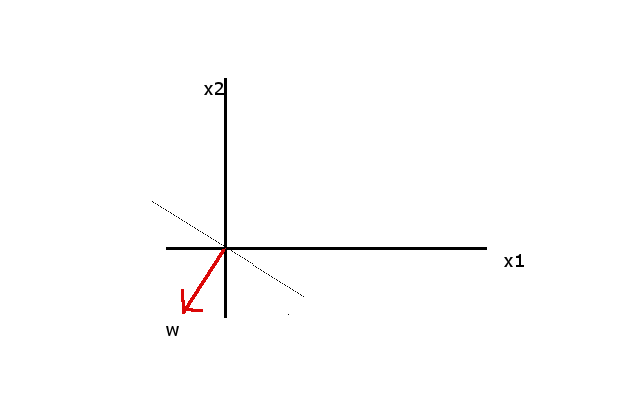
\includegraphics[width=15cm]{figures/graph4.png}
\end{center}

この状態で、最初の学習データとして$x^{(1)} = (125,30)$というデータが有ったとすると、まずはこれでパラメータを更新することを考える。

\begin{center}
  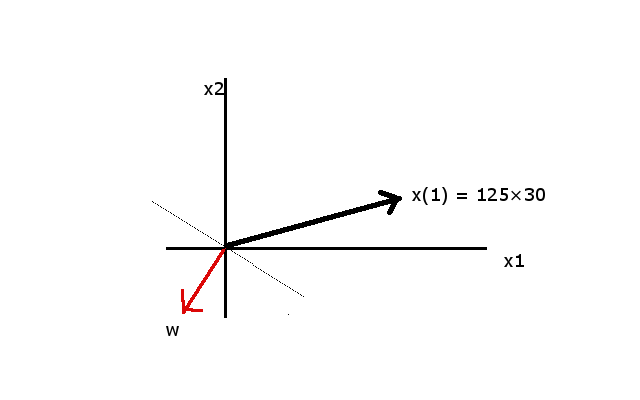
\includegraphics[width=15cm]{figures/graph5.png}
\end{center}

学習データのベクトル$x^{(1)}$に対して重みベクトルwはほぼ反対を向いている(内積が負)になっているので識別関数$f_w(x^{(1)})$による分類は-1になる。この学習データ$x^{(1)}$のラベル$y~{(1)}$は1だから、$f_w(x^{(1)}) \neq y^{(1)}$になって分類に失敗したという状態。

そして先程の更新式が適応される。

\begin{align}
	w + y^{(1)} x^{(1)} = w + x^{(1)}
 \end{align}
 
計算した結果、更新後の重みベクトルは以下のようになる。

\begin{center}
  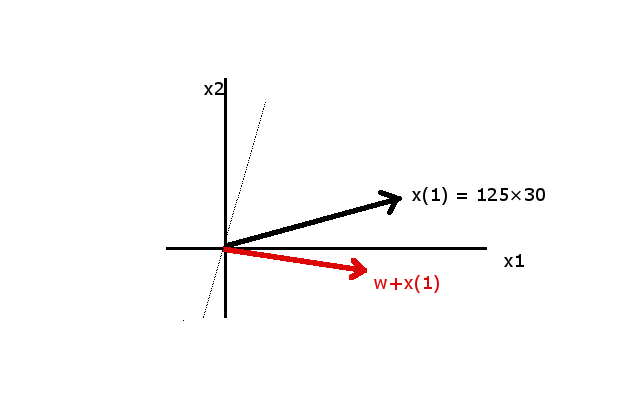
\includegraphics[width=15cm]{figures/graph6.png}
\end{center}

今度は$\theta < 90^\circ$になっているから、内積が性になって識別関数$f_w(x)$による分類は1になる。そして$x^{(1)}$のラベルも1だから、分類に成功したことがわかる。

この更新をすべての学習データについて繰り返していくのがパーセプトロンの学習である。

\subsection{線形分離可能}
パーセプトロンには「線形分離可能な問題しか解けない」という大きな問題がある。

\begin{center}
  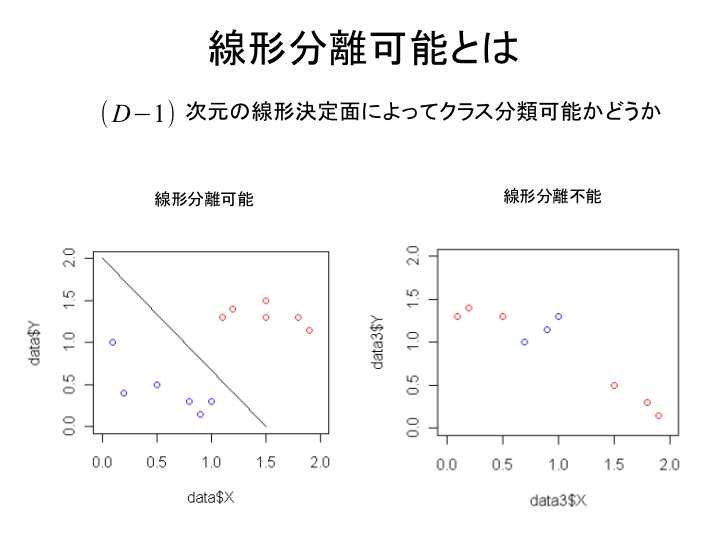
\includegraphics[width=15cm]{figures/graph7.jpg}
\end{center}

上の右図のように直線で分類できないものを「線形分離不能」という。

画像などを分類する際は、入力がとても高次元になるから可視化はできず、特徴を掴んで分類しようとするタスクはそれほど単純ではなく、殆どの場合が線形分離不可能に当たる。

これまで説明してきたパーセプトロンは、単純パーセプトロンや単層パーセプトロンと呼ばれる場合がある。それ単体だと貧弱なモデルだが、多層パーセプトロンと呼ばれるものがあり、それがニューラルネットワークである。これは非常に表現力が高いモデルであるが、今回は扱わない。

パーセプトロンとは異なるが、線形分離不可能な問題にも適応できるアルゴリズムが他に存在する。

\subsection{ロジスティック回帰}
先ほどと同じように、画像の横長と縦長を分類する例について考える。

分類を「縦長である確率が80\%、横長である確率が20\%」などと、確率として考えるというアプローチを取る。ここでは横長を1、縦長を0とする。1と0にするのは更新式を完結に書くため。実際は何でも良い。

\subsubsection{シグモイド関数}
回帰のときにパラメータ付きの以下のような式を使った

\begin{align}
	f_{\theta}(x) = \theta^{T}x
\end{align}

最急降下法か確率的勾配降下法を用いてパラメータの$\theta$を学習し、その$\theta$を使って未知のデータxに対する出力値を求めることができる。

ここでも考え方は同じで、未知のデータが度のクラスに分類されるかを求める関数$f_{\theta}(x)$が必要となる。パーセプトロンでの識別関数$f_w(x)$と役割は同じもの。

\begin{align}
	f_{\theta}(x) = \frac{1}{1+\exp(-\theta^{T}x)}
\end{align}

$\exp(-\theta^{T}x)$は指数関数を表す。$\exp(x)はe^x$と同じで「ネイピア数」と呼ばれる定数。2.7182...という値を持つ。

この関数は「シグモイド関数」といい、具体的には以下のような形をしている。

\begin{center}
  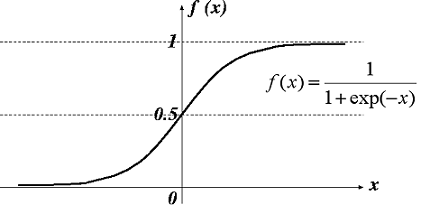
\includegraphics[width=15cm]{figures/graph8.png}
\end{center}

$\theta^{T}x=0のときにf_{\theta}(x)=0.5$になっており、$0 < f_{\theta}(x) < 1$というのがシグモイド関数の特徴。シグモイド関数は$0 < f_{\theta}(x) < 1$だから確率として扱える。

\subsubsection{決定境界}
以降から、未知のデータxが横長という確率を$f_{\theta}(x)$ということにする。

\begin{align}
	P(y=1|x) = f_{\theta}(x)
\end{align}

Pの中の縦棒は条件付き確率を表す。xというデータが与えられたときにy=1、つまり横長になる確率ということ。例えば$f_\theta(x)$を計算して0.7だったとすると、xは横長に分類されたということ。このように0.5をしきい値に分類することができるので、以下のように式を起こすことができる。

\begin{align}
	y = \left \{
    	\begin{array}{cc}
        1 & (\theta^{T}x \neq 0)\\
        0 & (\theta^{T}x < 0)
        \end{array}
    \right. \\
\end{align}

回帰のときと同じように$\theta$を適当に決めて具体的に考えてみる。例えば、$\theta$が以下のようなベクトルだったとき、$\theta^{T}x \geq 0$をグラフにしてみる。

\begin{align}
  	\bf{\theta} = \begin{pmatrix} 
      \theta_0\\
      \theta_1\\
      \theta_2
	\end{pmatrix}
    = \begin{pmatrix} 
      -100\\
      2\\
      1
	\end{pmatrix}
    ,
    \hspace{15pt}
    x = \begin{pmatrix} 
      1\\
      x_1\\
      x_2
	\end{pmatrix}
\end{align}

代入してわかりやすい形にすると、

\begin{align}
	\theta^{T}x = -100 \cdot 1 + 2x_1 + x_2 \geq 0 \\
    x_2 \geq -2_1 + 100
\end{align}

\begin{center}
  \includegraphics[width=15cm]{figures/graph9.png}
\end{center}

このようにデータを分類するための直線を「決定境界」という。

この決定境界は正しく分類されていないように見えるが、それば適当にパラメータをきめたため。回帰のときと同じように、正しいパラメータ$\theta$を決めるために目的関数を定義する必要がある。

\subsection{尤度関数}
xが横長である確率$P(y=1|x)をf_\theta(x)$と定義した。それを踏まえた上で、学習データのラベルyと$f_\theta(x)$はどのような関係にあるのが理想的か。

y=1のとき$f_\theta(x)=1$でy=0のとき$f_\theta(x)=0$になっているのが理想的であると言える。これは以下のように言い換えることができる。

\begin{itemize}
	\item{y=1のときは、確率$P(y=1|x)$が最大になってほしい}
    \item{y=0のときは、確率$P(y=0|x)$が最小になってほしい}
\end{itemize}

これをすべての学習データについて当てはめて行くと、最初に列挙した6個の学習データそれぞれに対して最大になってほしい確率は以下のようになる。

\begin{table}[htb]
  \begin{tabular}{|c|c|c|c|c|} \hline
    画像サイズ & 形 & y & 確率 \\ \hline
    80×150 & 縦長 & 0 & $P(y=0|x)$が最大になってほしい \\ \hline
    60×110 & 縦長 & 0 & $P(y=0|x)$が最大になってほしい \\ \hline
    35×130 & 縦長 & 0 & $P(y=0|x)$が最大になってほしい \\ \hline
    160×50 & 横長 & 1 & $P(y=1|x)$が最大になってほしい \\ \hline
    160×20 & 横長 & 1 & $P(y=1|x)$が最大になってほしい \\ \hline
    125×30 & 横長 & 1 & $P(y=1|x)$が最大になってほしい \\ \hline
  \end{tabular}
\end{table}

そして、すべての学習データはお互いに関係なく独立に発生すると考えると、この場合の全体の確率は以下のような同時確率で表せる。

\begin{align}
	L(\theta) = P(y^{(1)} =0|x^{(1)}) P(y^{(2)} =0|x^{(2)}) \cdots P(y^{(6)} =1|x^{(6)})
\end{align}

これは以下のように一般化してかける。

\begin{align}
	L(\theta) =\prod_{i=1}^{n} P(y^{(i)} = 1|x^{(i)})^{y^{(i)}} P(y^{(i)} = 0|x^{(i)})^{1-y^{(i)}}
\end{align}

これからはこの目的関数を最大化するパラメータ$\theta$を考える。ここでの$L(\theta)$は尤度とも呼ばれる。

\subsection{対数尤度関数}
パラーメタ$\theta$を求めるため、微分を施していくのだが、この尤度関数そのままでは扱いづらいため、微分する前に変形する。

確率はどれも1以下になるので同時確率ようのうような確率の掛け算はどんどん値が小さくなっていく。プログラミングする際には少数の制度問題も発生する。

そこで、尤度関数の対数を取ることにする。

\begin{align}
	\log L(\theta) &= \log \prod_{i=1}^{n} P(y^{(i)} = 1|x^{(i)})^{y^{(i)}} P(y^{(i)} = 0|x^{(i)})^{1-y^{(i)}} \\
    &= \sum_{i=1}^{n} (\log P(y^{(i)} = 1|x^{(i)})^{y^{(i)}} + \log P(y^{(i)} = 0|x^{(i)})^{1-y^{(i)}}) \\
    &= \sum_{i=1}^{n} ( {y^{(i)}} \log P(y^{(i)} = 1|x^{(i)}) + (1-y^{(i)}) \log P(y^{(i)} = 0|x^{(i)})) \\
    &= \sum_{i=1}^{n} ( {y^{(i)}} \log P(y^{(i)} = 1|x^{(i)}) + (1-y^{(i)}) \log (1-P(y^{(i)} = 1|x^{(i)}))) \\
    &= \sum_{i=1}^{n} (y^{(i)} \log f_\theta(x^{(i)}) + (1-y^{(i)}) \log (1-f_\theta(x^{(i)})))
\end{align}

今考えているのはy=1かy=0の2つしかないから$P(y^{(i)} = 0|x^{(i)}) + P(y^{(i)} = 1|x^{(i)}) = 1$になるはずである。確率はすべて足し合わせたら1になるから。

\subsubsection{尤度関数の微分}
ロジスティック回帰はこの対数尤度関数を目的関数として使うことになる。

\begin{align}
	\log L(\theta) = \sum_{i=1}^{n} (y^{(i)} \log f_\theta(x^{(i)}) + (1-y^{(i)}) \log (1-f_\theta(x^{(i)})))
 \end{align}

これをそれぞれのパラメータ$\theta_j$で微分していけば良い。

\begin{align}
	\frac{\partial \log L(\theta)}{\partial \theta_j} = \frac{\partial}{\partial \theta_j} \sum_{i=1}^{n} (y^{(i)} \log f_\theta(x^{(i)}) + (1-y^{(i)}) \log (1-f_\theta(x^{(i)}))
\end{align}

回帰のときと同じように、尤度関数を

\begin{align}
	u = \log L(\theta) \\
    v = f_\theta(x)
\end{align}

と置き換えて合成関数の微分を使う。

\begin{align}
	\frac{\partial u}{\partial v} = \frac{\partial u}{\partial v} \cdot \frac{\partial v}{\partial \theta_j}
\end{align}

まずは第一項目から計算する。

\begin{align}
	\frac{\partial u}{\partial v} &= \frac{\partial}{\partial v} \sum_{i=1}^{n} (y^{(i)} \log(v) + (1-y^{(i)}) \log(1-v) \\
    &= \sum_{i=1}^{n}(\frac{y^{(i)}}{v} - \frac{1-y^{(i)}}{1-v})
\end{align}

次にvを$\theta_j$で微分する。シグモイド関数の微分には以下のことが知られている。

\begin{align}
	\frac{d \sigma(x)}{dx} = \sigma(x)(1-\sigma(x))
\end{align}

また、$x=\theta^{T}x$とおいてもう一弾界、合成関数の微分を使う。

\begin{align}
	x = \theta^{T}x \\
    v = f_\theta(x) = \frac{1}{1+\exp(-x)} \\
    \frac{\partial v}{\partial \theta_j} = \frac{\partial v}{\partial z} \cdot \frac{\partial x}{\partial \theta_j}
\end{align}

これにより、

\begin{align}
	\frac{\partial v}{\partial \theta_j} &= \frac{\partial v}{\partial z} \cdot \frac{\partial z}{\partial \theta_j} \\
    &= v(1-v) \cdot x_j
\end{align}

以上のことから

\begin{align}
	\frac{\partial u}{\partial v} &= \frac{\partial u}{\partial v} \cdot \frac{\partial v}{\partial \theta_j} \\
    &= \sum_{i=1}^{n} (\frac{y^{(i)}}{v} - \frac{1-y^{(i)}}{1-v}) \cdot v(1-v) \cdot x_j^{(i)} \\
    &= \sum_{i=1}^{n} (y^{(i)}(1-v) - (1-y^{(i)})v)x_j^{(i)} \\
    &= \sum_{i=1}^{n} (y^{(i)} - y^{(i)}v - v + y^{(i)}v)x_j^{(i)} \\
    &= \sum_{i=1}^{n} (y^{(i)} - v ) x_j^{(i)} \\
    &= \sum_{i=1}^{n} (y^{(i)} - f_\theta(x^{(i)}))x_j^{(i)}
\end{align}

となる。あとはこの四季からパラメータ更新式を導出すれば良い。ただ、今は最大化することが目的だから、最小化のときとはパラメータを逆の方向にずらしていく必要がある。

\begin{align}
	\theta_j := \theta_j + \eta \sum_{i=1}^{n} (y^{(i)} - f_\theta(x^{(i)}))x_j^{(i)}
\end{align}

\end{document}
